\documentclass{school-22.211-notes}
\date{April 2, 2012}

\begin{document}
\maketitle

\lecture{Multi-Group Diffusion Derivations} \label{multi-group-diffusion}
\topic{Derivation of Multi-Group Diffusion Theory}
\begin{enumerate}
\item Start from the steady-state continuous energy diffusion equation, we divide the energy range into $G$ groups as shown in Figure~\ref{energy-groups}. 
\begin{figure}[ht]
  \centering
  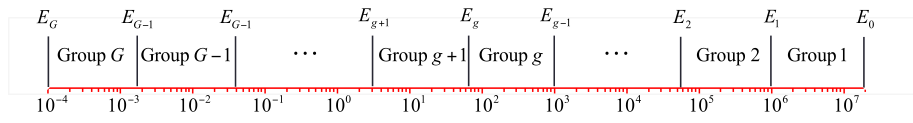
\includegraphics[width=6in]{images/dfs/energy-group.png}
  \caption{Energy Groups in Multi-Gruop Diffusion Theory} \label{energy-groups}
\end{figure}

\item Define group terms. We define the yet unknown group fluxes by the integrals of the flux over individual groups. \textcolor{blue}{Be careful about the units: $\phi_g(\vecr)$ is the real flux, $\phi(\vecr, E)$ is really the flux density}. Similarly the reaction rate is actually reaction rate density. This implementation does not have volume term in it because we are considering an infinite system. 
\eqn{ \phi_g(\vecr) = \int_{E_g}^{E_{g-1}} \phi(\vecr, E) \dE }
The group cross sections are defined such that the reaction rates in each interval are preserved,
\eqn{ \sigma_{xg}^i (\vecr) = \frac{1}{\phi_g (\vecr)} \int_{E_g}^{E_{g-1}} \sigma_x^i (\vecr, E) \phi(\vecr, E) \dE = \frac{\int_{E_g}^{E_{g-1}} \sigma_x^i (\vecr, E) \phi(\vecr, E) \dE}{\int_{E_g}^{E_{g-1}} \phi(\vecr, E) \dE} }
Group constants are typically determined using neutron spectra obtained by solving local problems with approximate boundary conditions, like our MC code. Group-wise cross sections cannot match the details of Monte Carlo spectrum calculation, so it is important that \textit{detailed resonance effects are contained in the multi-group cross sections} when produced from some detailed spectral calculations. For instance, we can approximate $\phi(E)$ using $\chi(E)$ for fast energies, using narrow resonances for intermediate energies, and Maxwellian distribution for the thermal energies. 



\item Integrate steady-state diffusion equation over each of the $g$ energy groups: 
\begin{align}
& - \overbrace{\int_{E_g}^{E_{g-1}} \dE \divergence D(\vecr, E) \gradient \phi(\vecr, E)}^{\mbox{leakage/diffusion term }\textcircled{1}} + 
\overbrace{\int_{E_g}^{E_{g-1}} \dE \Sigma_t(\vecr, E) \phi(\vecr, E)}^{\mbox{total interaction term }\textcircled{2}} = \overbrace{\int_{E_g}^{E_{g-1}} \dE S(\vecr, E)}^{\mbox{source term } \textcircled{3}}  \\
& + \overbrace{\int_{E_g}^{E_{g-1}} \dE \chi(E) \int_{E'} \dE' \nu \Sigma_f (\vecr, E') \phi(\vecr, E')}^{\mbox{fission source term }\textcircled{4}} 
 + \overbrace{\int_{E_g}^{E_{g-1}} \dE \int_{E'} \dE' \Sigma_s(\vecr, E'\to E) \phi(\vecr, E')}^{\mbox{scattering source term }\textcircled{5}} 
\end{align}

\item Simplify terms using group terms,
  \begin{enumerate}
  \item Leakage/Diffusion term: 
    \begin{align}
      \textcircled{1} &=\int_{E_g}^{E_{g-1}} \dE \divergence D(\vecr, E) \gradient \phi(\vecr, E) =  \divergence D_g(\vecr) \int_{E_g}^{E_{g-1}} \dE \gradient \phi(\vecr, E) = \divergence D_g (\vecr) \gradient \phi_g(\vecr) 
    \end{align}
    The group diffusion coefficient $D_g$ should be a tensor (a 3x3 symmetric matrix, called the Eddington tensor); but in application, we assume that $D_g$ is the same for all directions. That is, the tensor is approximated by a diagonal matrix (or call it current-weighted-diffusion-coefficient): 
    \eqn{ D_g^u (\vecr) = \frac{\int_{E_g}^{E_{g-1}} \dE D(\vecr, E) \ppu \phi(\vecr, E) }{\ppu \phi_g}, u = x,y,z} 
    It is not a great definition because for an infinite system $\ppu \phi = 0$ which would give us 0 over 0. A more accurate approach is to let $D_g$ be the same in the x-y plane, but different in axial direction. 

  \item Total interaction term: 
    \begin{align}
      \textcircled{2} &= \int_{E_g}^{E_{g-1}} \dE \Sigma_t(\vecr, E) \phi(\vecr, E) = \Sigma_{tg}(\vecr) \int_{E_g}^{E_{g-1}} \dE \phi(\vecr, E) = \Sigma_{tg} (\vecr) \phi_g(\vecr) 
    \end{align}
    where the macroscopic cross section is a sum over all isotropes $i$:
    \begin{align}
      \Sigma_{tg}(\vecr) &= \Sum_{i} N_i(\vecr) \sigma_{tg}^i (\vecr) \\
      \sigma_{tg}^i (\vecr) &= \frac{\int_{E_g}^{E_{g-1}} \sigma_t^i (E) \phi(\vecr, E) \dE }{\int_{E_g}^{E_{g-1}} \phi(\vecr, E) \dE}
    \end{align}
  \item Source term: 
    \eqn{ \textcircled{3} =\int_{E_g}^{E_{g-1}} \dE S(\vecr, E) =  S_g(\vecr) }

  \item Fission source term (this formation has only one fissioning species): 
    \eqn{ \textcircled{4} &=\int_{E_g}^{E_{g-1}} \dE \chi(E) \int_{E'} \dE' \nu \Sigma_f (\vecr, E') \phi(\vecr, E') =  \chi_g \Sum_{g'=1}^G \nu \Sigma_{fg} (\vecr) \phi_g(\vecr) }
        where 
        \eqn{ \chi_g &= \int_{E_g}^{E_{g-1}} \dE \chi(E), &\nu \sigma_{fg}^i (\vecr) &= \frac{1}{\phi_g(\vecr)} \int_{E_g}^{E_{g-1}} \nu(E) \sigma_f^i (E) \phi(\vecr, E) \dE }

  \item Scattering source term: 
  \begin{align}
    \textcircled{5} &=\int_{E_g}^{E_{g-1}} \dE \int_{E'} \dE' \Sigma_s(\vecr, E'\to E) \phi(\vecr, E') \\
    &= \int_{E_g}^{E_{g-1}} \dE \Sum_{g'=1}^G \int_{E_g'}^{E_{g'-1}} \dE' \Sigma_s(\vecr, E'\to E) \phi(\vecr, E') \\
    &= \Sum_{g'=1}^G \int_{E_g}^{E_{g-1}} \dE \int_{E_g'}^{E_{g'-1}} \dE' \Sigma_s(\vecr, E'\to E) \phi(\vecr, E') \\
    &= \Sum_{g'=1}^G \Sigma_{sg'g} (\vecr) \phi_{g'} (\vecr) 
  \end{align}
  where
  \eqn{\sigma_{sg'g}^i (\vecr) = \frac{1}{\phi_{g'} (\vecr) } \int_{E_g}^{E_{g-1}} \dE \int_{E_{g'}}^{E_{g'-1}} \dE' \sigma_s^i (E'\to E) \phi(\vecr, E') }

  \end{enumerate}

\item The Multi-Group Diffusion Equation is, 
\eqn{ -\divergence D_g(\vecr) \gradient \phi_g (\vecr) + \Sigma_{tg} (\vecr) \phi_g(\vecr) = \chi_g\Sum_{g'=1}^G \nu \Sigma_{fg'} \phi_{g'}(\vecr) + \Sum_{g'=1}^G \Sigma_{sg'g} (\vecr) \phi_{g'} (\vecr) + S_g(\vecr) }
Cancelling the within group scattering cross section from both sides and defining the group-wise \hi{net removal cross section}, 
\eqn{ \Sigma_{rg} = \Sigma_{tg} - \Sigma_{sgg} = \Sigma_{ag} + \Sum_{g'=1, g'\neq g} \Sigma_{sgg'} }
We obtain the final multi-group form of the neutron diffusion equation, 
\eqn{ \boxed{- \divergence D_g(\vecr) \gradient \phi_g(\vecr) + \Sigma_{rg} (\vecr) \phi_g(\vecr) = \chi_g \Sum_{g'=1}^G \nu \Sigma_{fg'} (\vecr) \phi_{g'} (\vecr) + \Sum_{g'=1,g'\neq g}^G \Sigma_{sg'g} (\vecr) \phi_{g'} (\vecr) + S_g(\vecr) } }
\end{enumerate}
Notes:
\begin{itemize}
\item A note about the \uline{summation sign}: the loss terms do not need to be summed over energy groups because once a neutron leaves group $g$ it does not matter where it goes, whereas the gain terms need to be summed over energy groups to take into account all neutrons contributing from every other energy group. 

\item A note about the \uline{sign of the leakage term}: the absolute value of leakage always have a negative sign. 
  \begin{itemize}
  \item Typically RHS $>0$ (we have either fission, scattering, or source), then the curve is concave down. We can either think about it in terms of second derivative, which is negative; or we can think the slope is decreasing, which means that $\laplacian \phi < 0$. The heat transfer analogy is that when there are sources everywhere in the slab, there would be heat transfer away at every point. 
    
  \item In the extreme case RHS $<0$ , and the system is losing neutrons due to absorption or scattering out, then the flux would be concave up, meaning $\laplacian \phi > 0$. The heat transfer analygo is that when there are sinks everywhere in the slab, there would be heat transfer inwards at every point. 

  \item When RHS $=0$, the flux would be a straight line, $\gradient \phi = $ constant, $\laplacian \phi = 0$, there is no leakage/diffusion at every point, that is, there is no net neutrons leaving any point, the neutron diffusion breakes even at every point. The heat transfer analogy is that there is no heat leaving or entering any point. 
  \end{itemize}
\end{itemize}


\clearpage
\topic{Matrix Form}
If we keep the destruction terms on the LHS, and the construction terms on the RHS,
\begin{align}
\left[ \begin{array}{cccc} 
    - D_1 \laplacian +  \Sigma_{r1} & & & \\
    & -D_2 \laplacian  +  \Sigma_{r2} & & \\
    & & \ddots & \\
    & & &  - D_G \laplacian + \Sigma_{rG}  \end{array} \right] 
\left[ \begin{array}{c} \phi_1 \\ \phi_2 \\ \vdots \\ \phi_G \end{array} \right]\\
= \left[ \begin{array}{cccc} 
\frac{\chi_1 \nu \Sigma_{f1}}{k} & \Sigma_{s21} + \frac{\chi_1 \nu \Sigma_{f2}}{k} & \cdots &  \Sigma_{sG1} + \frac{\chi_1 \nu \Sigma_{fG}}{k} \\
\Sigma_{s12} + \frac{\chi_2 \nu \Sigma_{f1}}{k} & \frac{\chi_2 \nu \Sigma_{f2}}{k} & \cdots &  \Sigma_{sG2} + \frac{\chi_2 \nu \Sigma_{fG}}{k} \\
\vdots & & \ddots &  \\
\Sigma_{s1G} + \frac{\chi_G \nu \Sigma_{f1}}{k} & \Sigma_{s21} + \frac{\chi_1 \nu \Sigma_{f2}}{k} & \cdots & \frac{\chi_1 \nu \Sigma_{fG}}{k} \\
\end{array} \right] 
\left[ \begin{array}{c} \phi_1 \\ \phi_2 \\ \vdots \\ \phi_G \end{array} \right]
\end{align}
Alternatively, we can move the scattering terms to the LHS, 
\begin{align}
\left[ \begin{array}{cccc} 
    - D_1 \laplacian +  \Sigma_{r1} & - \Sigma_{s21} & \cdots & - \Sigma_{sG1} \\
    - \Sigma_{s12} & -D_2 \laplacian  +  \Sigma_{r2} & \cdots & - \Sigma_{sG2} \\
    \vdots & \vdots & \ddots & \vdots \\
    - \Sigma_{s1G} & - \Sigma_{s21} & \cdots &  - D_G \laplacian + \Sigma_{rG}  \end{array} \right] 
\left[ \begin{array}{c} \phi_1 \\ \phi_2 \\ \vdots \\ \phi_G \end{array} \right]
= \left[ \begin{array}{cccc} 
\frac{\chi_1 \nu \Sigma_{f1}}{k} & \frac{\chi_1 \nu \Sigma_{f2}}{k} & \cdots & \frac{\chi_1 \nu \Sigma_{fG}}{k} \\
\frac{\chi_2 \nu \Sigma_{f1}}{k} & \frac{\chi_2 \nu \Sigma_{f2}}{k} & \cdots &   + \frac{\chi_2 \nu \Sigma_{fG}}{k} \\
\vdots & & \ddots &  \\
\frac{\chi_G \nu \Sigma_{f1}}{k} & \frac{\chi_1 \nu \Sigma_{f2}}{k} & \cdots & \frac{\chi_1 \nu \Sigma_{fG}}{k} \\
\end{array} \right] 
\left[ \begin{array}{c} \phi_1 \\ \phi_2 \\ \vdots \\ \phi_G \end{array} \right]
\end{align}
Notes: we have the $k$ term in the equations to keep the fission source general. In the absence of spatial dependency (for instance, in this formulation we've only considered energy dependency so far and assume spatial homogenization), notice the RHS matrix has order 1 (this can be seen from that every row vector is a constant times the 1st row), leading to that there is only one eigenvalue, thus we do not have to worry about multiple eigenvalues. This implies that \hi{the eigenvalue is a measurement of the spatial dependency}. Once we add in the flux depending on both space and energy, we cannot easily write each row as the 1st row times a constant anymore. 



\clearpage
\topic{Partial Currents}
\begin{enumerate}
\item Scalar flux, 
  \eqn{\phi(\vecr, E) = \int_{4\pi} \psi(\vecr, E, \vecOmega) \dOmega }
\item Net current,
  \eqn{\vecJ(\vecr, E) = \int_{4\pi} \vecOmega \psi(\vecr, E, \vecOmega) \dOmega  }
\item Partial Currents in diffusion theory:
  \begin{align}
    J^+(\vecr, E) &= \int_{\vecn \cdot \vecOmega > 0} \vecn \cdot \vecOmega \psi(\vecr, E, \vecOmega) \dOmega \\
    &= \frac{1}{4\pi} \int_{\vecn \cdot \vecOmega > 0} \vecn \cdot \vecOmega [\phi(\vecr, E) + 3 \vecOmega \cdot \vecJ(\vecr, E) ] \dOmega \\
    &= \frac{1}{4\pi} \int_0^{2\pi} \dphi \int_0^1 \dmu [ \mu \phi + 3 \mu^2 J_n] \\
    &= \frac{1}{4} \phi(\vecr, E) + \frac{1}{2} J_n (\vecr, E) \\
    J^-(\vecr, E) &= \int_{\vecn \cdot \vecOmega < 0} |\vecn \cdot \vecOmega| \psi(\vecr, E, \vecOmega) \dOmega  \\
    &= -\frac{1}{4\pi} \int_0^{2\pi} \dphi \int_{-1}^0 \dmu [ \mu \phi + 3 \mu^2 J_n] \\
    &= \frac{1}{4} \phi(\vecr, E) - \frac{1}{2} J_n (\vecr, E) 
  \end{align}

\item A common expansion for angular flux (I think this is second order) from Reuss: 
\eqn{    \int_{4\pi} \psi \dOmega &= \phi }
\eqn{    \int_{4\pi} \Omegahat \psi \dOmega &= \vec{J} }
\eqn{    \Rightarrow \psi &= \frac{1}{4\pi} \left[ \phi + 3 \Omegahat \cdot \vec{J} \right] }
\end{enumerate}

\end{document}
